\def\layersep{2.5cm}
% https://texample.net/tikz/examples/neural-network/
\begin{figure}
    \centering
    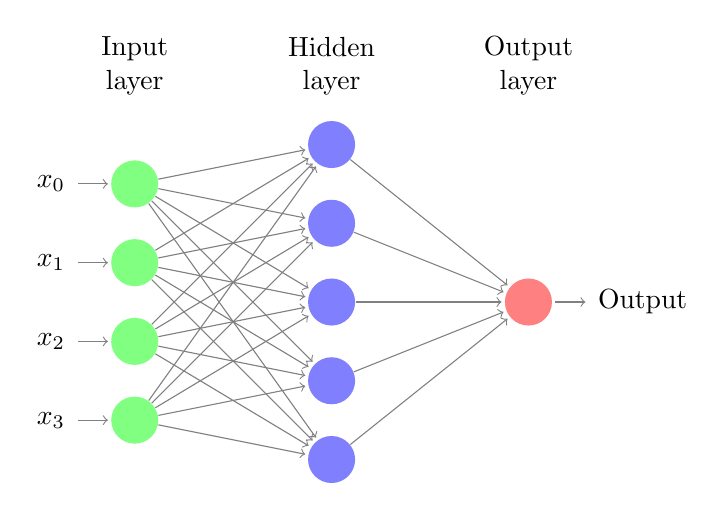
\begin{tikzpicture}[shorten >=1pt,->,draw=black!50, node distance=\layersep]
        \tikzstyle{every pin edge}=[<-,shorten <=1pt]
        \tikzstyle{neuron}=[circle,fill=black!25,minimum size=17pt,inner sep=0pt]
        \tikzstyle{input neuron}=[neuron, fill=green!50];
        \tikzstyle{output neuron}=[neuron, fill=red!50];
        \tikzstyle{hidden neuron}=[neuron, fill=blue!50];
        \tikzstyle{annot} = [text width=4em, text centered]
        
        % Draw the input layer nodes
        \foreach \name / \y in {0,...,3}
        % This is the same as writing \foreach \name / \y in {1/1,2/2,3/3,4/4}
        \node[input neuron, pin=left: $x_{\y}$] (I-\name) at (0,-\y) {};
        
        % Draw the hidden layer nodes
        \foreach \name / \y in {0,...,4}
        \path[yshift=0.5cm]
        node[hidden neuron] (H-\name) at (\layersep,-\y cm) {};
        
        % Draw the output layer node
        \node[output neuron,pin={[pin edge={->}]right:Output}, right of=H-2] (O) {};
        
        % Connect every node in the input layer with every node in the
        % hidden layer.
        \foreach \source in {0,...,3}
        \foreach \dest in {0,...,4}
        \path (I-\source) edge (H-\dest);
        
        % Connect every node in the hidden layer with the output layer
        \foreach \source in {0,...,4}
        \path (H-\source) edge (O);
        
        % Annotate the layers
        \node[annot,above of=H-0, node distance=1cm] (hl) {Hidden layer};
        \node[annot,left of=hl] {Input layer};
        \node[annot,right of=hl] {Output layer};
    \end{tikzpicture}
    \caption{\label{fig:theory-mlp}An example of a simple, feed-forward neural network architecture. Each input
    $x_i$ is fed to each node in the hidden layer, where the value of the activation
    function $f(z)$ is calculated and passed on to the output layer. In this case the
    output layer consists of only one node.
    }
\end{figure}